\section{Power-Stage Structure}
\label{sec:analysis-overview}

The reference LED converter's separate pump and isolated resonant paths \cite{ammar2021led} were implemented in the prototype. The bridge provides the rectified input, the pump charges the high-voltage link, and the GaN half bridge drives the isolated output network. Figure~\ref{fig:analysis-power-stage} shows the common power paths using the V2 schematic.



The rectified input follows the mains envelope, while the DC link stores energy and supplies the half bridge. Pump capacitance \(\CP\), inductance \(\LP\), and steering/clamp paths transfer energy between these nodes during each enabled cycle.

The isolated branch is excited from \texttt{VSW} through series capacitance \(\CRES\), discrete inductance, and transformer leakage. The transformer includes a separate magnetizing branch; secondary rectification supplies the bulk capacitor and MPQ4242 stage. \(V_{\mathrm{sec}}\) is the secondary bulk voltage, and VBUS is the USB-C output voltage.

Signed branch currents sum at the half bridge and jointly determine device current and commutation. The DC link couples collected pump power to secondary demand over longer intervals.

The active carrier remains at \SI{1}{\mega\hertz}; burst duration is controlled by PA10 on the original prototype. Secondary-bulk feedback \(V_{\mathrm{sec}}\) enters PA1, optional primary-voltage feed-forward enters PA0, and primary-current feedback at PA2 distinguishes loaded and no-load states. Burst control changes both average secondary transfer and pump charge-transfer density.

\begin{landscape}
\begin{figure}[H]
    \centering
    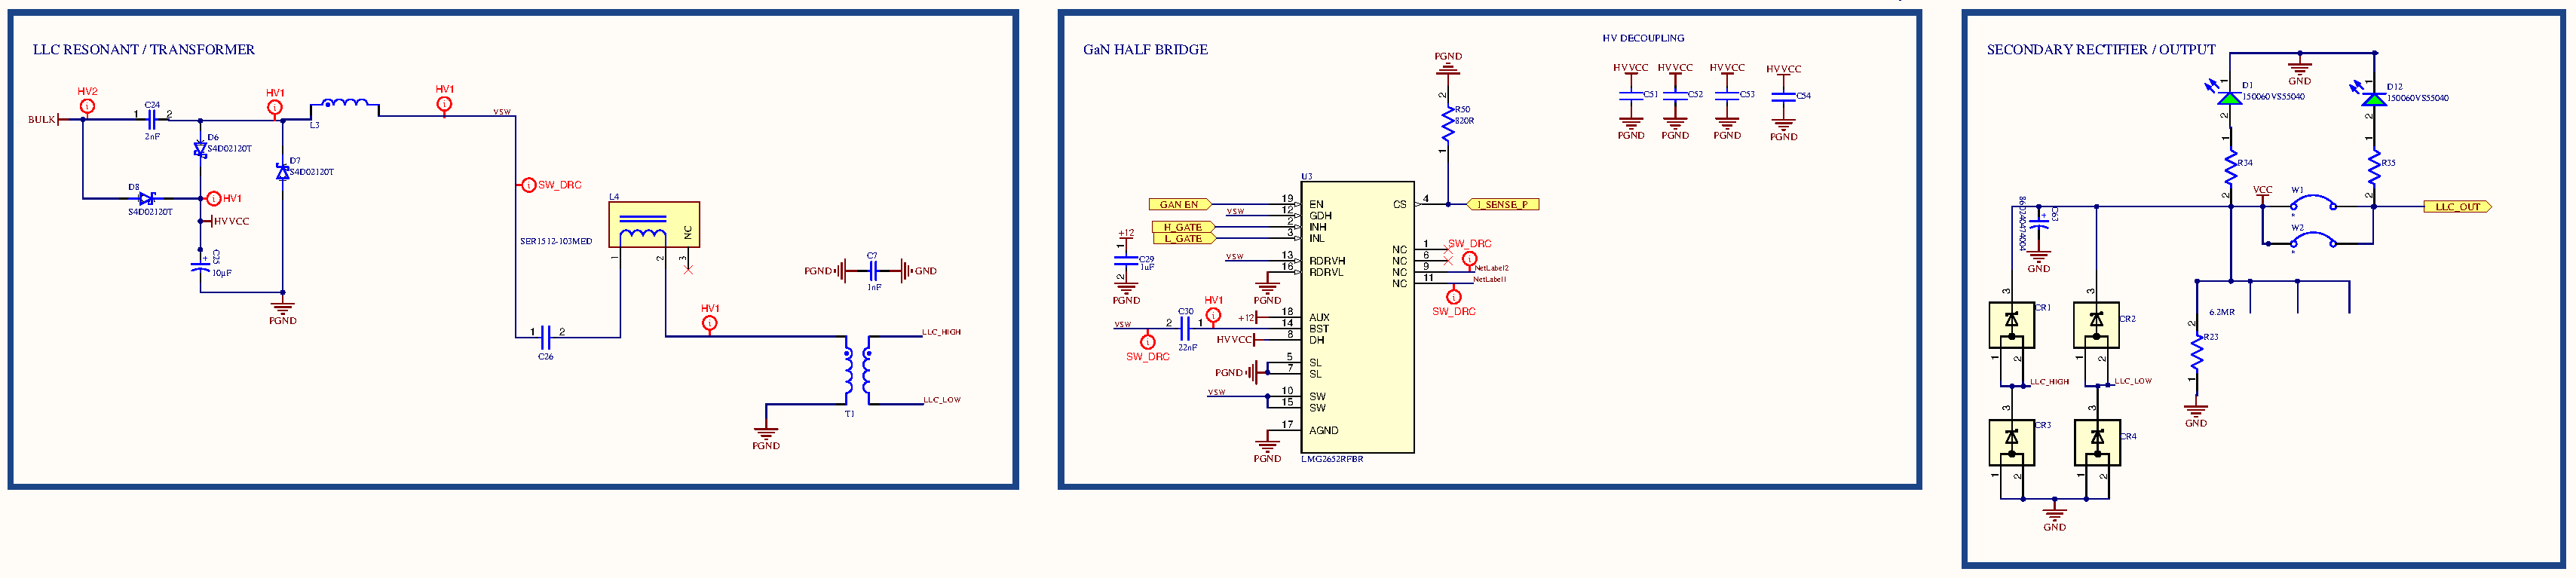
\includegraphics[width=0.97\linewidth,height=0.82\textheight,keepaspectratio]{Pictures/Thesis/07_Hardware/Rebuilt/schematic_v2_power_stage_excerpt.pdf}
    \caption{V2 sheet 3 power paths: charge-pump branch, GaN half bridge, resonant tank and transformer, and secondary rectifier.}
    \label{fig:analysis-power-stage}
\end{figure}
\end{landscape}
